% SIAM Article Template
\documentclass[review,onefignum,onetabnum]{siamart190516}

% Information that is shared between the article and the supplement
% (title and author information, macros, packages, etc.) goes into
% ex_shared.tex. If there is no supplement, this file can be included
% directly.
% SIAM Shared Information Template
% This is information that is shared between the main document and any
% supplement. If no supplement is required, then this information can
% be included directly in the main document.


% Packages and macros go here
\usepackage{lipsum}
\usepackage{amsfonts}
\usepackage{graphicx}
\usepackage{epstopdf}
\usepackage{algorithmic}
\usepackage[T1]{fontenc}
\usepackage[utf8]{inputenc}
\ifpdf
  \DeclareGraphicsExtensions{.eps,.pdf,.png,.jpg}
\else
  \DeclareGraphicsExtensions{.eps}
\fi

% Add a serial/Oxford comma by default.
\newcommand{\creflastconjunction}{, and~}

% Used for creating new theorem and remark environments
\newsiamremark{remark}{Remark}
\newsiamremark{hypothesis}{Hypothesis}
\crefname{hypothesis}{Hypothesis}{Hypotheses}
\newsiamthm{claim}{Claim}

% Sets running headers as well as PDF title and authors
\headers{Adaptive methods using GP for regret-based estimates}{V. Trappler, E. Arnaud, A. Vidard}

% Title. If the supplement option is on, then "Supplementary Material"
% is automatically inserted before the title.
\title{Adaptive methods using GP for regret-based estimates\thanks{Document compiled on \today }% \thanks{Submitted to the editors DATE.
% \funding{This work was funded by the Fog Research Institute under contract no.~FRI-454.}}
}

% Authors: full names plus addresses.
\author{Victor Trappler\thanks{Univ. Grenoble-Alpes  (\email{victor.trappler@univ-grenoble-alpes.fr}, \url{http://vtrappler.github.io/}).}
\and Elise Arnaud \thanks{Univ Grenoble-Alpes} \and Arthur Vidard\footnotemark[3]}

\usepackage{amsopn}
\DeclareMathOperator{\diag}{diag}
\newcommand{\kk}{\theta}
\newcommand{\uu}{u}
\newcommand{\KK}{\theta}
\newcommand{\UU}{U}
\newcommand{\Kspace}{\Theta}
\newcommand{\Uspace}{\mathbb{U}}
\newcommand{\Xspace}{\mathbb{X}}
\newcommand{\Prob}{\mathbb{P}}
\newcommand{\Ex}{\mathbb{E}}
\newcommand{\argmin}{\mathrm{arg}\,\mathrm{min}}
\newcommand{\argmax}{\mathrm{arg}\,\mathrm{max}}
%%% Local Variables: 
%%% mode:latex
%%% TeX-master: "ex_article"
%%% End: 


% Optional PDF information
\ifpdf
\hypersetup{
  pdftitle={Adaptive methods using GP for regret-based estimates},
  pdfauthor={V. Trappler, E. Arnaud, and A. Vidard}
}
\fi

% The next statement enables references to information in the
% supplement. See the xr-hyperref package for details.

\externaldocument{ex_supplement}

% FundRef data to be entered by SIAM
%<funding-group specific-use="FundRef">
%<award-group>
%<funding-source>
%<named-content content-type="funder-name"> 
%</named-content> 
%<named-content content-type="funder-identifier"> 
%</named-content>
%</funding-source>
%<award-id> </award-id>
%</award-group>
%</funding-group>


\graphicspath{{/home/victor/collab_article/adaptive/figures/}}

\begin{document}

\maketitle

% REQUIRED
\begin{abstract}
  This is an example SIAM \LaTeX\ article. This can be used as a
  template for new articles.  Abstracts must be able to stand alone
  and so cannot contain citations to the paper's references,
  equations, etc.  An abstract must consist of a single paragraph and
  be concise. Because of online formatting, abstracts must appear as
  plain as possible. Any equations should be inline.
\end{abstract}

% REQUIRED
\begin{keywords}
  example, \LaTeX
\end{keywords}

% REQUIRED
\begin{AMS}
  68Q25, 68R10, 68U05
\end{AMS}

\section{Introduction}
\subsection{Contextual introduction}
\label{sec:context}

For many applications, many decisions must be taken.

\lipsum[2-3]

However, uncertainties have to be taken into account, as optimality
may not be carried when some uncertain conditions change.  The
objective function is then represented as a random variable, that we
wish to minimize in some sense.

% The outline is not required, but we show an example here.

\cite{trappler_robust_2020}
\subsection{Optimisation under uncertainties, regret}
\label{sec:problem-definition}
In the field of decision under uncertainties,
\cite{savage_theory_1951} proposes the notion of regret,
where each outcome is compared to the best outcome possible.

\begin{definition}[Regret]
 For a function $f: \Xspace \rightarrow \mathbb{R}$, we define the regret $r$ as
\begin{align}
  r_{\mathrm{A}}(x) &= f(x) - \min_{x\in\Xspace} f(x) = f(x) - f^* \\
  r_{\mathrm{R}}(x) &= \frac{f(x)}{\min_{x\in \Xspace}f(x)} = f(x)/f^* = \frac{f(x) - f^*}{f^*} + 1
\end{align}
where the subscript A refers to an \emph{additive} regret, while the
subscript R refers to the \emph{relative} regret. 
\end{definition}



In this work, we consider having an objective function $J$. Defined
contextually, this function usually represents a risk, or a cost
associated with its argument. De facto, decision leading to low values
of $J$ are sought by the user.

In the context of decision under uncertainty, we are going to consider that the input can be split in
two different components
\begin{itemize}
\item First, the control variable $\kk\in\Kspace$, whose choice is up to the user 
\item Secondly, the environmental variable $\uu \in \Uspace$
\end{itemize}

\begin{equation}
  \label{eq:J_def}
  \begin{array}{rcl}
    \Kspace \times \Uspace  &  \longrightarrow & \mathbb{R} \\
    (\kk, \uu) & \longmapsto & J(\kk, \uu)
  \end{array}
\end{equation}
The environmental variable is an additional variable, which represents
some \textit{uncontrollable} parameters, or, in other words,
parameters that cannot be tuned, due to their intrinsic variability.
In order to transcribe this uncertainty on the environmental variable,
we choose to model it as a random variable $\UU$ while $\uu\in\Uspace$
belongs to its sample space.

In this work, we assume that the distribution of $\UU$ is known and
that we can get samples from it.  We also consider that the objective
function is completely deterministic, as the sampling of $\UU$ is up
to the user, before the evaluation of $J$.



From an optimisation point of view, we then want $J$ to be as small as
possible, regardless of the sample of the environmental variable
$\uu$. In this work, we propose to use the notions of regret, in order
to define objectives for the robsut optimization of this objective function.



\section{Estimates based on the regret}
\label{sec:estim-based-regr}

As $J$ takes two inputs, we can then define the regret in this case:

\begin{definition}[Regret]
\begin{align}
  r_{\mathrm{A}}(\kk, \uu) &= J(\kk, \uu) - \min_{\kk\in\Kspace} J(\kk, \uu) = J(\kk, \uu) - J^*(\uu) \\
  r_{\mathrm{R}}(\kk, \uu) &= \frac{J(\kk, \uu)}{\min_{\kk\in \Kspace}J(\kk, \uu)} = J(\kk, \uu)/ J^*(\uu)
\end{align}
where $J^*: \uu \mapsto J^*(\uu)$ is the conditional minimiser, or
profile optimiser in~\cite{ginsbourger_bayesian_2014}.
\end{definition}
By accounting for the random nature of $\UU$, the regret is also a
random variable, indexed by $\kk \in \Kspace$. In this work, we focus on the quantiles of this random variable, defined as:
\begin{equation}
  q_p(\kk) = Q_{\UU}(r(\kk, \UU);p) = \inf_{\alpha} \left\{\Prob_{\UU}\left[r(\kk, \UU)\leq \alpha \right] \geq p\right\}
\end{equation}
In other words, this quantile is the smallest value which bounds the
regret with probability at least $p$.  A value of $\kk$ which provides
robustness is then linked to a small $\alpha$, and a large probability
$p$.  For that purpose we will then put the emphasis on the comparison
of the regret with specific thresholds.  More precisely, on the
estimation of quantities involving affinely the conditional minimum:
\begin{equation}
  J(\kk, \uu)  - \alpha J^*(\uu) - \beta 
\end{equation}
where $\alpha$ and $\beta$ are chosen appropriately depending on
whether the additive or the relative regret is considered.

However, in most problems, $J$ is quite expensive to evaluate
computational wise, and limiting its evaluations is crucial if not
mandatory. The specific case of robust optimization is even more
problematic, as it requires an exploration with respect to the sample
space of $\UU$, and an estimation of the conditional minimisers.

Because of that, we propose to use Gaussian Processes in order to
compute these quantities, and by using their properties, we can select
new points to evaluate in order to improve the estimations.

\section{GP formulation of regret-based problems}
\label{sec:GP_formul}
\subsection{Kriging equations}
\label{sec:krigin_eq}
Let us assume that the objective function $J$ has been first evaluated on an
initial design $\mathcal{X}_0$ defined as
\begin{equation}
  \mathcal{X}_0 = \left\{\left(x_1,J(x_1)\right),\dots,\left(x_{n_0},J(x_{n_0})\right)\right\} \in \left(\Xspace \times \mathbb{R} \right) ^{n_0}
\end{equation}
where for the sake of brievety, when no distinction between $\kk$ and $\uu$ is needed, $x_i = (\kk_i, \uu_i)$ for $1 \leq i \leq n_0$, and $\Xspace = \Kspace \times \Uspace$.
This design is usually chosen with space-filling properties, such as Latin Hypersquare samples.
The set of evaluations are abbreviated as
\begin{align}
  \mathbf{x} &= (x_1, \dots, x_{n_0})\in \Xspace^{n_0} \\
  \mathbf{z} &= J(\mathbf{x}) = \left(J({x}_1),\dots, J(x_{n_0})\right) \in \mathbb{R}^{n_0}
\end{align}
The GP constructed using the initial design is then written as
\begin{equation}
  Z \mid \mathcal{X}_0 \sim \mathrm{GP}(m_{Z\mid\mathcal{X}_0}, C_{Z \mid \mathcal{X}_0})
\end{equation}
where $m_{Z\mid \mathcal{X}_0}$ can be interpreted as a surrogate of
$J$, and $C_{Z\mid \mathcal{X}_0}$ is the covariance function chosen
to represent the function. Popular choices of covariance functions
include Gaussian (assuming $C^\infty$), Exponential (assuming $C^1$
differentiability), or Matérn 5/2 (assuming $C^2$
differentiability). The parameters of this function are usually chosen
by maximum likelihood.  In order to derive the expression of
$m_{Z\mid\mathcal{X}_0}$, we can consider the joint distribution of
the already evaluated points $\mathbf{x}$, and the random process at
an unevaluated point $x$:
\begin{equation}
  \begin{pmatrix}
    Z(\mathbf{x}) \\
    Z(x)
  \end{pmatrix}
  \sim \mathcal{N}\left(
    \begin{pmatrix}
      \mu_Z \\ m_{Z\mid\mathcal{X}_0}(x)
    \end{pmatrix} ;
    \begin{pmatrix}
      \mathbf{K}_{\mathcal{X}_{n_0}} & K_{\mathcal{X}_{n_0}}(x) \\
      K_{\mathcal{X}_{n_0}}(x)^T  & C_Z(x,x)
    \end{pmatrix}
    \right)
\end{equation}
\begin{align}
  Z(\mathbf{x}) &= \left(Z(x_1),\dots,Z(x_{n_0})\right) \\
  K_{\mathcal{X}_{n_0}}(x) &= \left(C_{Z\mid\mathcal{X}_0}(x, x_1), \dots, C_{Z\mid\mathcal{X}_0}(x, x_{n_0})\right) \\
  \mathbf{K}_{\mathcal{X}_{n_0}} &= \left(C_{Z\mid\mathcal{X}_0}(x_i, x_j) \right)_{1 \leq i,j \leq n_0}
\end{align}
where $\mu_Z$ is the prior assumption on the GP $Z$.

The kriging prediction is defined as
\begin{align}
  m_{Z \mid \mathcal{X}_{n_0}}(x) = \mu_Z(x) + K_{\mathcal{X}_{n_0}}^T \mathbf{K}_{\mathcal{X}_{n_0}}^{-1} \left( \mathbf{z} - \mu_Z(x)\right)
\end{align}
when the experimental design is clear from the context, it will be
dropped from the notation.
More specifically, we have that for any $x\in\Xspace$,
\begin{equation}
  Z(x) \sim \mathcal{N}\left(m_Z(x), \sigma_Z^2(x)\right)
\end{equation}
where $\sigma^2_Z(x) = C_Z(x, x)$


Given a design $\mathcal{X}$ and a GP, we can define a measure of the
prediction error associated with the conditioned GP by integrating the
prediction variance over the whole space. This is the Integrated Mean
Square Error (IMSE) (+ref)
\begin{equation}
  \label{eq:IMSE_def}
  \mathrm{IMSE}(Z \mid \mathcal{X}) = \int_{\Xspace} \sigma^2_{Z \mid \mathcal{X}}(x)\,\mathrm{d}x
\end{equation}


\subsection{Regret}
In order to use the notion of regret, we have first to going to model
$J^*$ using $Z$: we consider the plug-in approximation of the
conditional minimum:
\begin{equation}
  m_Z^*(\uu) = \min_{\kk \in \Kspace} m_Z(\kk, \uu) = m_Z(\kk_Z^*(\uu),\uu)
\end{equation}
where $\kk^*_Z(\uu)$ is the conditional minimiser.

The joint distribution of $Z(\kk,\uu)$ and $Z(\kk^*(\uu), \uu)$ can then be written as
\begin{equation}
  \begin{pmatrix}
    Z(\kk, \uu) \\
    Z\left(\kk^*(\uu), \uu\right)
  \end{pmatrix}
  \sim
  \mathcal{N}\left(
    \begin{pmatrix}
      m_Z(\kk, \uu) \\
      m^*_Z(\uu)
    \end{pmatrix};
    \begin{pmatrix}
      \sigma^2_Z(\kk, \uu) & C\left((\kk, \uu),(\kk^*(\uu),\uu)\right) \\
      C\left((\kk, \uu),(\kk^*(\uu),\uu)\right)&  \sigma^2_{Z^*}(\uu) \\
    \end{pmatrix}
  \right)
\end{equation}
Finally, by scaling the random vector $\begin{pmatrix}
  Z(\kk, \uu) \\
  Z\left(\kk^*(\uu), \uu\right)
\end{pmatrix}$ by $\begin{bmatrix} 1 & - \alpha \end{bmatrix}$ and
translating by $-\beta$, we can define the random process $\Delta$,
indexed over $\Kspace \times \Uspace$ as
\begin{align}
  \Delta(\kk, \uu) & = Z(\kk, \uu) - \alpha Z^*(\uu) - \beta
\end{align}
As a linear combination of GP, $\Delta$ is a GP as well, and thus, at each point $(\kk, \uu) \in \Kspace \times \Uspace$,
\begin{align}
\Delta(\kk, \uu) \sim  \mathcal{N}\left(m_\Delta(\kk, \uu);\sigma^2_\Delta(\kk, \uu) \right)
\end{align}
where the mean and variance function are
\begin{align}
  m_{\Delta}(\kk, \uu) &= m_Z(\kk, \uu) - \alpha m_Z^*(\uu) - \beta \\
  \sigma^2_{\Delta}(\kk, \uu) &= \sigma^2_Z(\kk, \uu)  + \alpha^2  \sigma^2_{Z^*}(\uu) - 2 \alpha C\left((\kk, \uu),(\kk^*(\uu),\uu)\right)
\end{align}
The prediction uncertainty associated with $\Delta$ stems from
\begin{itemize}
\item the uncertainty associated with the prediction error of $Z$
\item the uncertainty associated with the uncertainty on the conditional minimiser $Z^*$
\end{itemize}
\section{Exploration of the input space}
In this section, we will define and compare some exploration
strategies.  Let us say that the GP has been conditioned on a design
comprising $n$ points: $\mathcal{X}_n$.  In a myopic strategy, the
next point is chosen by defining and optimising a criterion $\kappa$.
\begin{align}
  x_{n+1} = \argmin_{x\in\Xspace} \kappa(x ; Z\mid \mathcal{X}_n) \\
  \mathcal{X}_{n+1} = \mathcal{X}_n \cup \{\left(x_{n+1}, J(x_{n+1})\right) \}
\end{align}
\subsection{Maximum variance exploration}
\label{sec:max_variance}
At a point $x \in \Xspace$, the uncertainty of the
prediction is measured by the variance $\sigma_Z^2(x)$.
In a greedy way, we can look to evaluate the point which presents the largest variance, \emph{i.e.}
\begin{equation}
  x_{n+1} = \argmax_{x\in\Xspace} \sigma^2_{Z\mid \mathcal{X}_n}(x)
\end{equation}

However, such procedure is adapted only if evaluating the point with
high variance will reduce this uncertainty. The uncertainty on the
estimation of $\Delta_{\alpha}$ stems from two sources, the lack of
knowledge of the function $J$, and the lack of knowledge of $J^*$. We
propose then to enrich the design by reducing globally the uncertainty
on $\Delta_{\alpha}$.

\subsection{Augmented IMSE}

Let $\mathcal{X}$ be a design, we say that this design is
augmented by the couple $(x, z)$, when we append the pair
point/evaluation $(x, z)$:
\begin{equation}
  \mathcal{X} \cup \left\{(x, z)\right\}
\end{equation}
The evaluation $z$, which is supposed to represent $J(x)$, is not yet
known, but we do have the knowledge that $z \sim Z(x)$.

By defining a criterion $\kappa$ which measures the uncertainty
associated with the design $\mathcal{X}\cup \left\{(x, z)\right\}$, and by averaging this criterion with respect to $Z(x)$, we can define

\begin{align}
  \mathbb{E}_{Z(x)}\left[\kappa(\mathcal{X} \cup \{(x, Z(x))\} \right] = \int_{\mathbb{R}} \kappa(\mathcal{X} \cup \{(x, z)\} \phi\left(\frac{z - m_Z(x)}{\sigma_Z(x)}\right) \,\mathrm{d}z
\end{align}
Finally, by choosing the IMSE as $\kappa$, the (expected) augmented
IMSE can be written as
\begin{align}
  \mathrm{aIMSE}(x) &= \Ex_{Z(x)}\left[\mathrm{IMSE}\left(\mathcal{X}\cup \{(x, Z(x))\}\right)\right] \\ &=\int_{\mathbb{R}} \left(\int_{\Xspace} \sigma^2_{\Delta\mid \mathcal{X} \cup \{(x, z)\}}(\xi) \, \mathrm{d}\xi \right) \phi\left(\frac{z - m_Z(x)}{\sigma_Z(x)}\right) \,\mathrm{d}z
\end{align}

The augmented IMSE can then be used as a criterion in order to select
the new point to be evaluated, in the sense that minimizing the aIMSE
means that we choose the point which produces the design with
the lowest IMSE on average.

Visually, we can see on Figure~\ref{fig:enrichment} that adding points with respect to this design, the exploration of the input space is twofold: there are points added near the predicted conditional minimisers (which reduce $\sigma^2_{Z^*}$), and other points which explore more the input space (in order to reduce $\sigma_Z^2$).
\begin{figure}[ht]
  \centering
  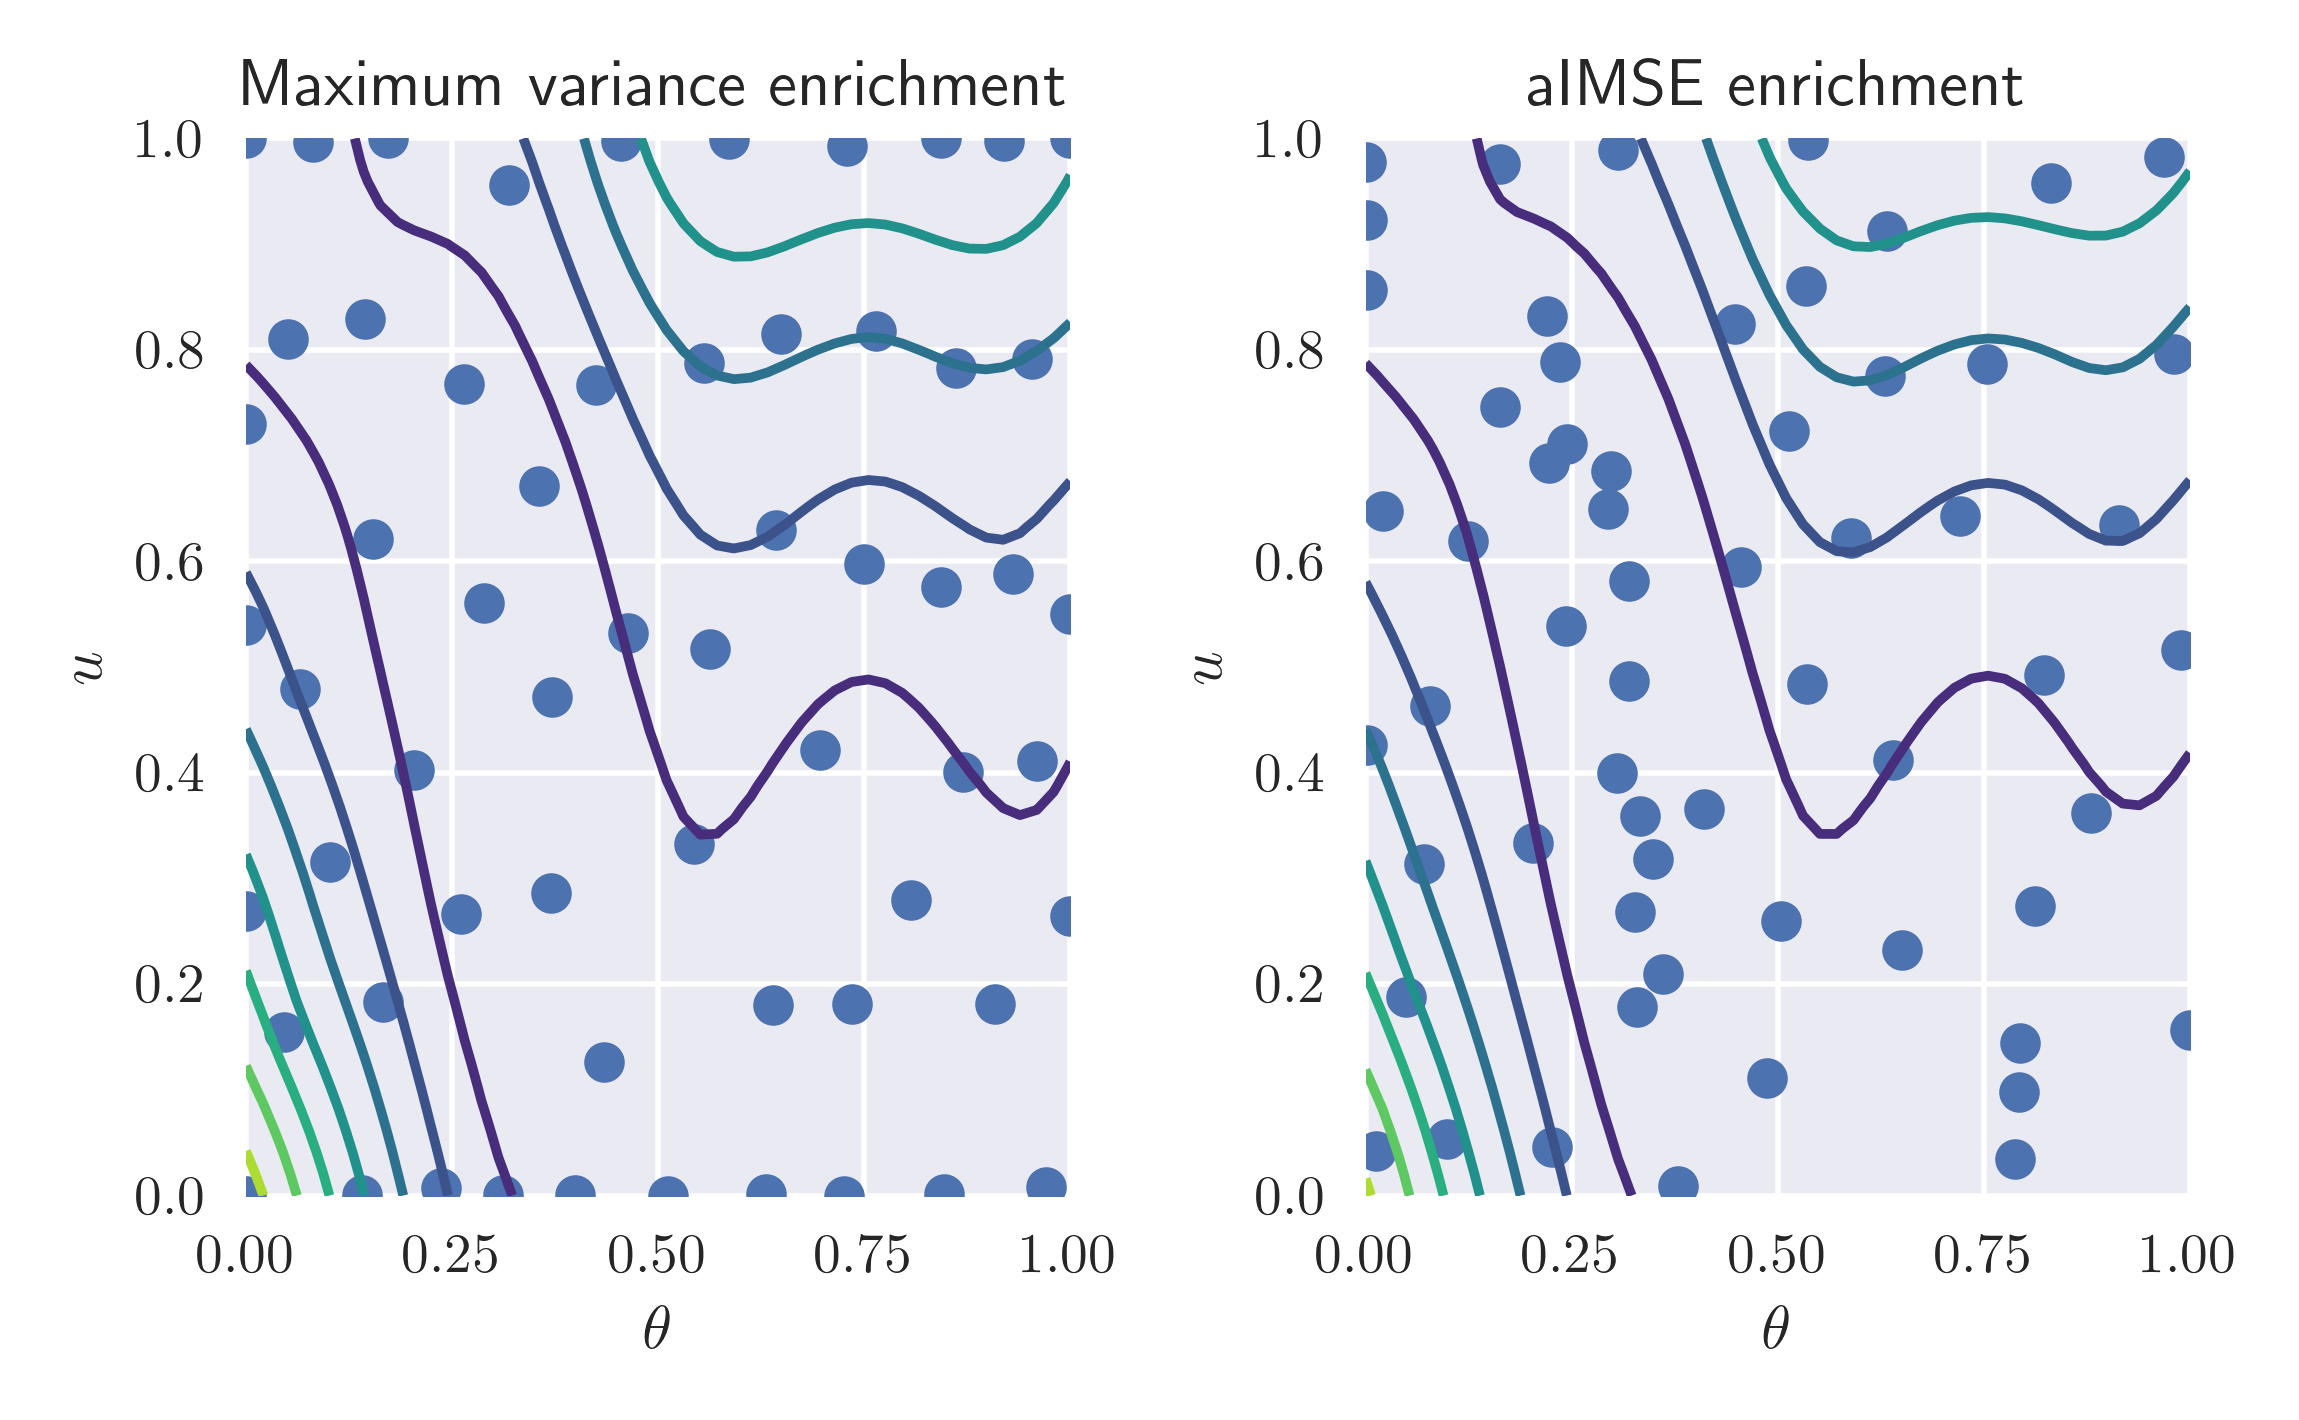
\includegraphics[width=\textwidth]{enrichment.png}
  \caption{\label{fig:enrichment} Comparison of the design after 50 points added to the design}
\end{figure}



\begin{figure}[ht]
  \centering
  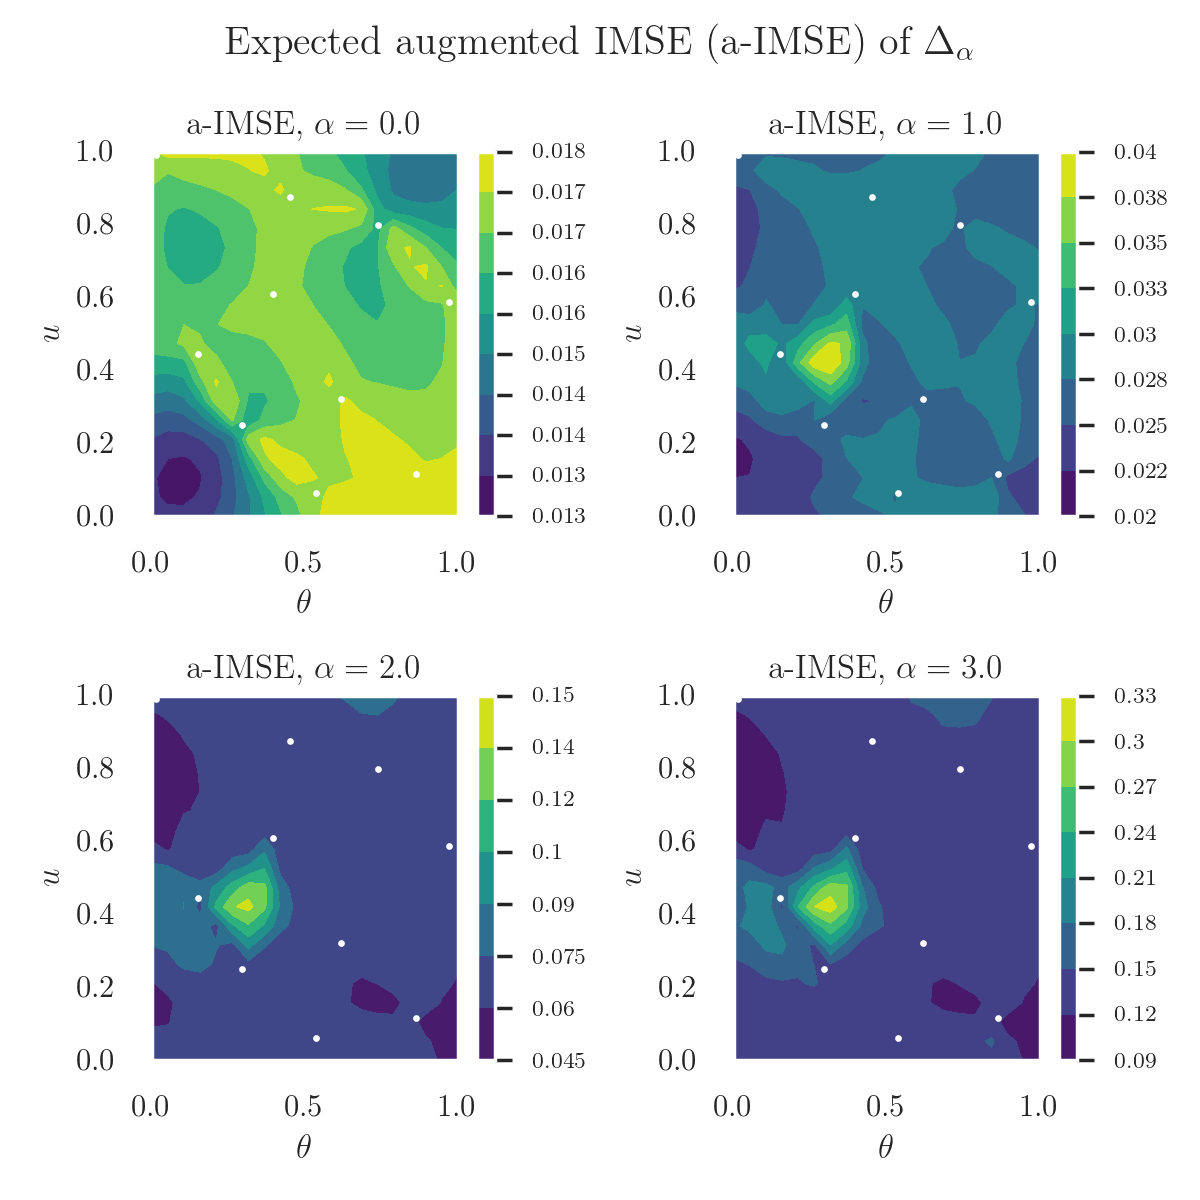
\includegraphics[width=\textwidth]{aIMSE_diff_alpha.png}
  \caption{\label{fig:aIMSE_diff_alpha} Expected augmented IMSE of
    $\Delta_{\alpha}$ for different $\alpha$. The case $\alpha=0$
    corresponds to the augmented IMSE of $Z$}
\end{figure}


\begin{figure}[ht]
  \centering
  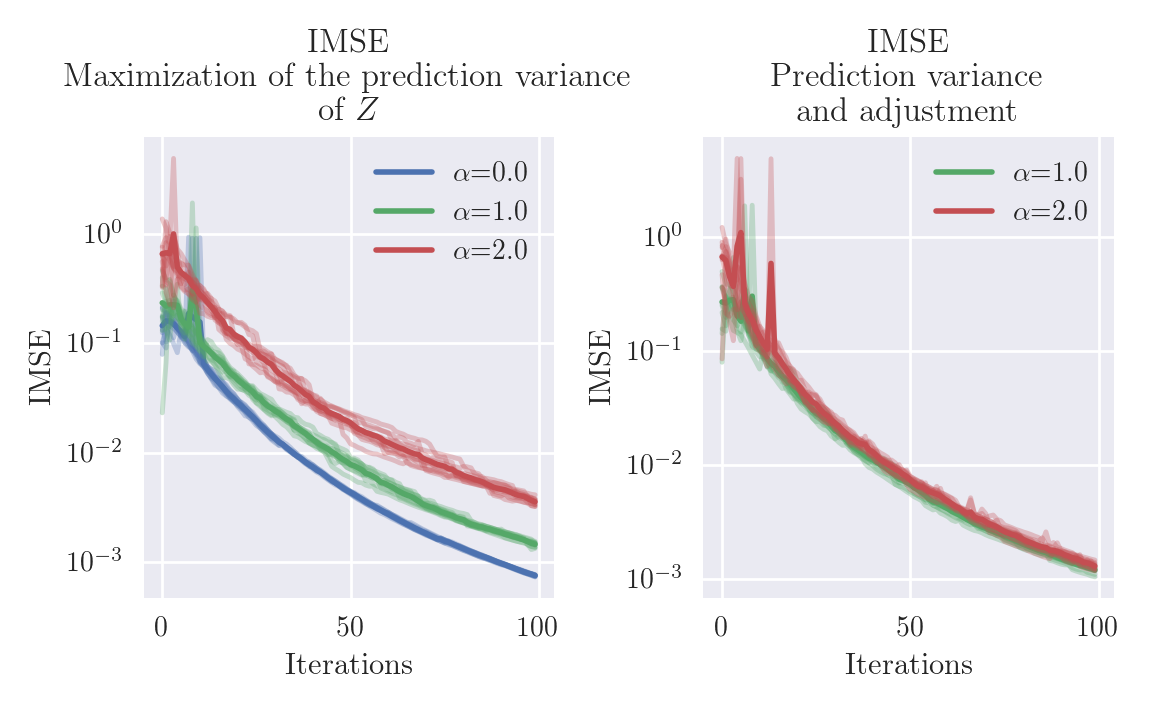
\includegraphics[width=\textwidth]{IMSE_predictionvariance_Delta_adjustment.png}
  \caption{\label{fig:IMSE_predictionvariance} }
\end{figure}


\section{Two-stage myopic method}


\section{Conclusions}
\label{sec:conclusions}

Some conclusions here.


\appendix
\section{An example appendix} 
azfgf



\section*{Acknowledgments}
We would like to acknowledge the assistance of volunteers in putting
together this example manuscript and supplement.

\bibliographystyle{siamplain}
\bibliography{/home/victor/acadwriting/bibzotero}
\end{document}
